\lab{Applications}{Filtering and Convolution}{Filtering and Convolution}
\objective{This lesson demonstrates the use of the Fourier Transform for cleaning up noisy signals and finding convolutions of signals.}

\section*{Cleaning up a noisy signal}

Listen to \texttt{Noisysignal1.wav} (see Figure \ref{noisysignal}). This is a mono recording of a (probably familar) voice with some annoying noise over it. Fortunately for us, this noise is ``colored", i.e. it only occurs over a limited range of frequencies. This makes it possible for us to remove it fairly easily without unduly damaging the underlying signal.
\begin{figure}[ht]\caption{Noisy signal}\label{noisysignal}\centering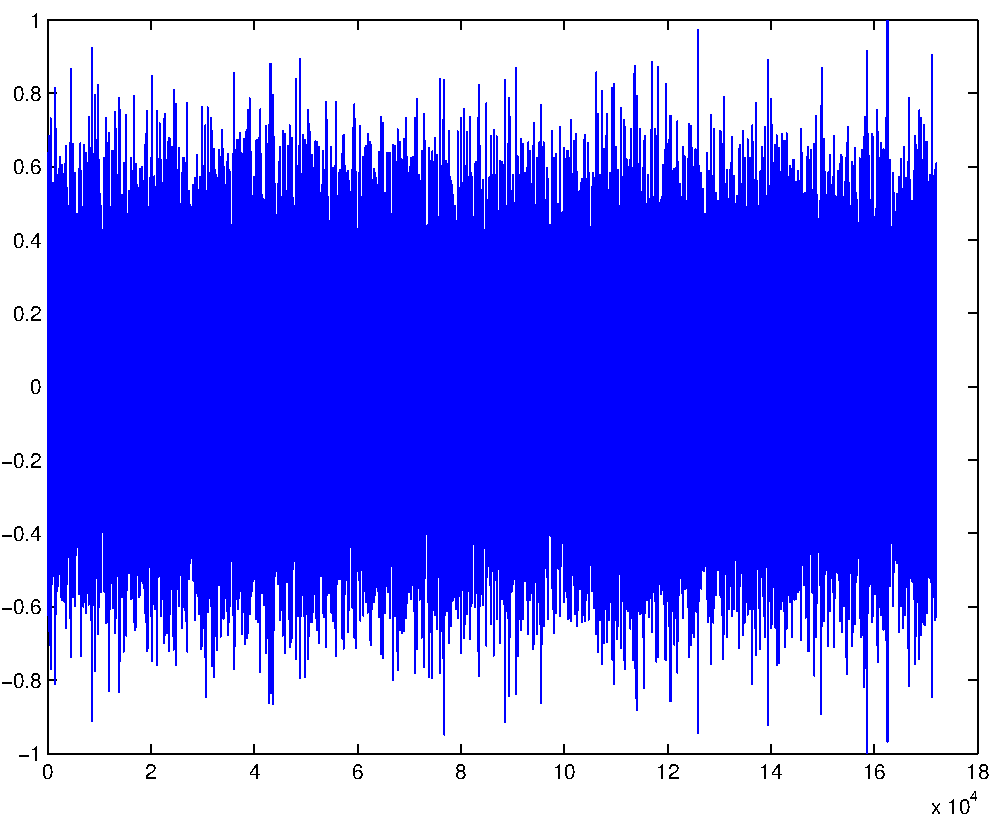
\includegraphics[width=\textwidth]{noisy}\end{figure}
How do we begin? First we examine the DFT of the signal in order to identify which frequencies make up the noise (see Figure \ref{noisyspec}).
\begin{figure}[ht]\caption{Spectrum of noisy signal}\label{noisyspec}\centering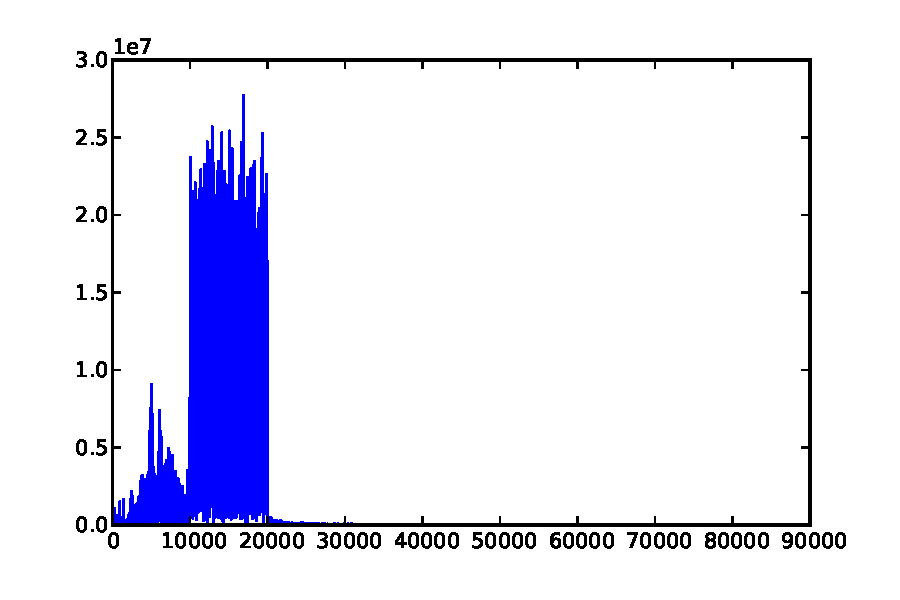
\includegraphics[width=\textwidth]{noisyspec}\end{figure}
We notice a large band from 10000 to 20000 units which seems to be intruding in the spectrum. This is our noise. (The fact that it begins and ends so abruptly in the spectrum, instead of tapering off gradually, should be a clue that this noise was produced artificially, by the author of this lab, rather than arising in a natural way in the recording or transmission process.) To remove the noise, we simply zero out this part of the DFT and then take the inverse DFT (using the function \texttt{anfft.ifft}) to get our cleaned-up signal. But we must remember to zero out the corresponding part in the right half of the DFT as well, in order to ensure that the inverse DFT of the result is a real-valued signal.

It is critical that the values zeroed in the right half of the DFT be precisely the mirror images of the zeroed in the left half: i.e., assuming the DFT of the signal is stored in the vector \texttt{fsig}, if we set \texttt{fsig[j]} to zero then we should also set \texttt{fsig[-j]} to zero. If we are off on the index even just by one, then the result will not be a real valued signal and thus will not be playable.

So, we do the whole thing in Python like this:
\begin{lstlisting}
rate,data = wavfile.read('Noisysignal1.wav')
fsig = sp.fft(data,axis = 0)
for j in xrange(10000,20000):
    fsig[j]=0
    fsig[-j]=0

newsig=sp.ifft(fsig)
newsig = sp.real(newsig)
newsig = sp.int16(newsig/sp.absolute(newsig).max() * 32767)
\end{lstlisting}

Now we can either save the resulting cleaned-up signal \texttt{newsig} to a \texttt{.wav} file using \texttt{wavwrite}. If we plot it, the individual syllables are now visible in the waveform (see Figure \ref{cleansignal}).

\begin{figure}[ht]\caption{Cleaned-up \texttt{Noisysignal1.wav} }\label{cleansignal}\centering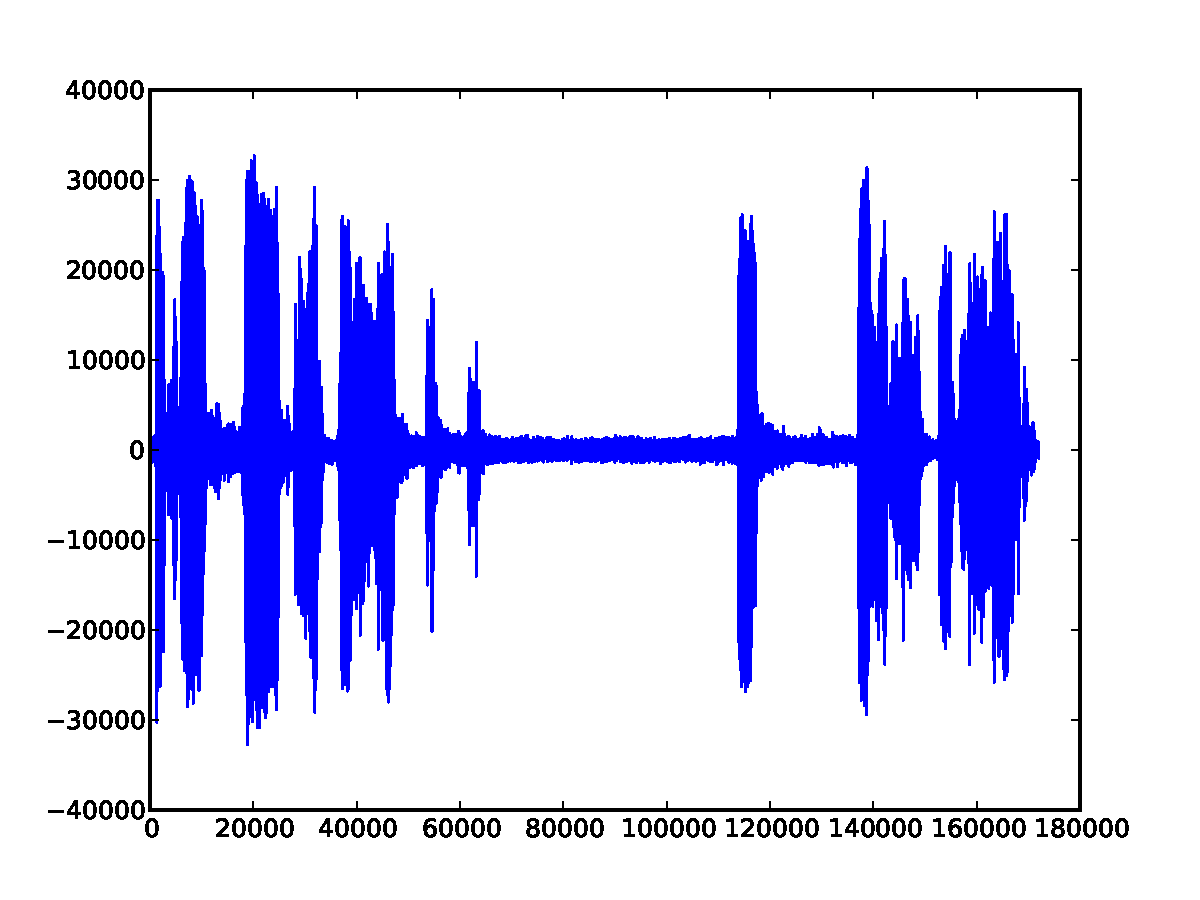
\includegraphics[width=\textwidth]{Cleanedsignal}\end{figure}

\begin{problem}
Listen to \texttt{Noisysignal2.wav}. You will probably just hear noise. However, there is a signal behind it. Remove the noise using the technique described above. In order to make the cleaned-up signal audible. What does the voice say? Who is the speaker? (If you don't know the answer to this last question, try a quick Google search.)
\end{problem}


\section*{Filtering and Convolution}

We have already seen how the DFT can be used to filter out certain bands of frequencies from a signal. In this section we will look at how the DFT can be used to carry out another type of filtering effect. To begin, suppose we have a recording of musical piece played in, say, a small carpeted room with essentially no acoustics, and suppose we would like to apply an effect to make it sound as if the piece were played in a large concert hall (or some other room). How could we do that?

The first thing we need is a recording of the so-called \emph{impulse response} of the room whose acoustics we are trying to imitate. This is a recording of how the room responds to a short pulse of sound. Effective ways of producing a loud sound approximating a pulse include firing a (blank) gunshot, popping a balloon, or, if neither of those are available, clapping the hands one time. You have probably noticed (or can imagine) that if you pop a balloon in large room, although the sound of the actual pop only lasts a few milliseconds, you can hear the sound echoing about the room for up to several seconds. This echoing sound is called the impulse response of the room. Actually, it is somewhat imprecise to refer to \emph{the} impulse response of the room, since the recorded response can significantly depend both on the location of device producing the pulse and on location of the listener (or recording device) in the room.

Now, the idea is that if we know how the room responds to a pulse, then we can reconstruct how the room will respond to any sound. This is because any sound can be considered to be a series of pulses of varying amplitudes and polarity (i.e., they may be positive or negative). Each sample of sound can be considered as a pulse, even though the ear will not perceive it that way, because the pulses are so close together. Now, we make the assumption that the room's response is linear, meaning that a pulse of $k$ times the amplitude will produce a response of $k$ times the amplitude but otherwise identical; such an assumption is generally reasonably accurate, assuming the pulse is not extremely loud. To calculate how the room responds to a complex sound consisting of millions of samples, we simply add up its response to each sample of the sound, each such response simply being a scaled copy of the impulse response which we recorded.

Thus, in our simulation, each sample of our sound (of which there are usually 44100 per second) triggers a new scaled copy of the room's impulse response. If the impulse response is several seconds long, that means there may be a hundred thousand or more scaled copies of the impulse response sounding at once, which must all be mixed together to produce the final sound. This may be starting to seem computationally infeasible or at least very difficult. The key is to recognize that this process can be described as a convolution: namely, the final sound is simply the convolution of the our original sound with the impulse response. We can calculate convolutions quickly using the convolution theorem which says

\[\mathcal{F}(f \ast g) = (\mathcal{F} f) (\mathcal{F} g)\]

where $\mathcal{F}$ is the Fourier Transform and $\ast$ is convolution.

Thus we calculate the convolution of two arrays by simply taking the fourier transform of each, multiplying them pointwise, and then taking the inverse transform.

\begin{problem}
\emph{This Problem is optional.  If the instructor does not require it then students may use the provided \texttt{balloon.wav} file which contains the sound of a balloon pop in a large room.}

Find a large room or area with good acoustics, and record (an approximation to) its impulse response using a balloon pop. To record the sound, you will want to use at least a decent microphone. You may want to record it using the program Audacity \footnote{Audacity is free software and may be downloaded at http://audacity.sourceforge.net} and a laptop. If you use a unidirectional microphone, be sure the microphone is pointing at the balloon when you pop it, so that the direct sound from the pop is picked up. (If you don't, the result will still be okay. It's just that after we do the convolution, it will probably sound somewhat distant, as if we are at the back of the room, where we can't hear the music directly, only through the reverberation of the room.)
If you've chosen a good room, the response should be audible for at least a full second.

Include a plot of both the waveform and spectrum of the impulse response you recorded.
\end{problem}


\begin{problem}\label{convolution_problem}
Download and listen to the file \texttt{chopinw.wav}. You will hear a piano being played in a dead room with little or no acoustics. Using the Convolution Theorem, take the convolution of this signal with the impulse response recorded in the previous problem. Describe the resulting sound.

In doing this problem, keep in mind that the Convolution Theorem requires both signals to have the same length; therefore you will need to pad the smaller of your two signals (namely, the impulse response signal) with zeros at the end in order to make it the same size as the other signal. But the convolution of the Convolution Theorem is a circular convolution, which will mean that the room's response to a sound near the end of the signal will wrap around back to the beginning of the signal in the result. In order to avoid this undesired effect, you will want to also pad the signals with additional zeros (at least as many zeros as one less than the size of the impulse response signal).
\end{problem}

In doing the preceding problem, keep in mind that the Convolution Theorem requires both signals to have the same length; therefore you will need to pad the smaller of your two signals (namely, the impulse response signal) with zeros at the end in order to make it the same size as the other signal. But the convolution of the Convolution Theorem is a circular convolution, which will mean that the room's response to a sound near the end of the signal will wrap around back to the beginning of the signal in the result. In order to avoid this undesired effect, you will want to also pad the signals with additional zeros (at least as many zeros as one less than the size of the impulse response signal).

In some instances, a circular convolution is actually desirable. For instance, an interesting effect is achieved by taking the circular convolution of a long segment of white noise with some other (shorter) sound. We can create white noise using scipy's \texttt{rand} function:
\begin{lstlisting}
#samplerate = 22050
#noise = sp.int16(sp.random.randint(-32767,32767,samplerate*10)) # Create 10 seconds of mono white noise
\end{lstlisting}

\begin{problem}
Create white noise in this way this and listen to the resulting sound (CAUTION: Turn your volume way down.  It may be very very loud).  This kind of noise is called ``white" because it contains all frequencies (below the Nyquist frequency) with the same strength, or rather, with the same expected strength (since the amplitude of a specific frequency is a matter of chance). In order to see this, plot the spectrum of the noise.
\end{problem}

Now we are going to take the circular convolution of this noise with some other sound. For instance, let's use \texttt{Tada.wav}. The result is in \texttt{tada-conv.wav}. We notice that the original short sound has been sustained to an indefinite length. The result is not a set of static tones, but rather a rich sound which preserves not only the tones, but the texture, of the original sound; you can hear different tones fluctuating randomly in amplitude over time. If you were to play this \texttt{tada-conv.wav} on repeat, you would find that, because we used a circular convolution, the sound loops seamlessly from the end back to the beginning; however, most sound players are not capable of doing this properly, so you will probably hear a break in the sound. To demonstrate the ``seamlessness", we can paste together three copies of the sound consecutively:

\begin{lstlisting}
rate, sig = wavfile.read('tada-conv.wav')
sig = sp.append(sig,sig)
sig = sp.append(sig,sig)
\end{lstlisting}

Listen to the resulting sound, and notice that we are not able to identify where the sound loops back to the beginning, because there is no break or click.

\begin{problem}
Record yourself singing a few notes (or, feel free to produce some other sound another way). Take the circular convolution of white noise with this recording. Now do it again using stereo white noise, which you can create, e.g., by doing \texttt{noise = sp.float16(sp.random.randint(-32767,32767,(samplerate*10,2)))}. It's no problem that your original recording will probably be mono; just make the left and right channels duplicate in the recording (but: be sure to use different left and right channels for the white noise). Can you hear any difference between the mono and stereo versions of the result?
\end{problem}

Feel free to play around with this. The file \texttt{guitar-conv.mp3} is a collage of sounds created using this technique (mostly using guitar samples). You could probably think of other lots of other things you can do with this.


%\begin{problem}
%Using the algorithm described in the lecture notes, implement your own Inverse Fast Fourier Transform (IFFT) in MATLAB from scratch. You may assume that $N$ is a power of 2. Test it on several random vectors and make sure the results match those of MATLAB's \texttt{ifft}. It should have $O(N\log N)$ running time. Now, by adjusting your IFFT, implement the FFT, and redo Problem \ref{convolution_problem} using the FFT and IFFT which you have implemented. Use \texttt{tic} and \texttt{toc} to measure how long it takes to finish, against how long it took using MATLAB's \texttt{fft} and \texttt{ifft}.
%\end{problem}
%
%It is possible to implement your \texttt{fft} and \texttt{ifft} using vector operations, which will speed things up; however, one could hardly expect to beat MATLAB's \texttt{fft} and \texttt{ifft}, which are implemented by calling the extremely well-optimized FFTW library (Fastest Fourier Transform in the West).



